%\chapter{det-comp}

%%%%%%%%%%%%%%%%%%%%%%%%%%%%%%%%%%%%%%%%%%%%%%
\section{Cryostat and feedthroughs}

%%%%%%%%%%%%%%%%%%%%%%%%%
\subsection{Scope and requirements}
\fixme{This may need some massaging to put `scope and req' at the beginning of this section}

The cryostat consists of a steel warm outer structure, layers of insulation and an inner cold membrane.  The outer %steel warm 
structure (shown in Figure~\ref{fig:warm-vessel-layout}), which provides %represents 
the mechanical support for the  %inner membrane cold cryostat 
membrane and its insulation,  consists of vertical beams that alternate with a web of metal frames. It is constructed to %capable of 
withstand the hydrostatic pressure of the liquid argon, the pressure of the gas volumes and %all possible 
satisfies the external constraints. %The steel warm structure for NP04 is shown in Figure~\ref{fig:warm-vessel-layout}.
In particular, this structure is to be constructed in EHN1 without any mechanical attachment to the floor or the building side walls.  \fixme{what are the ext constraints? Also, the text on the figure is too small; is it intended to indicate what each color is? Can you clarify and make sure each part/color is labeled?}
%
\begin{cdrfigure}[Warm vessel layout]{warm-vessel-layout}{Warm vessel layout showing the various major components}
  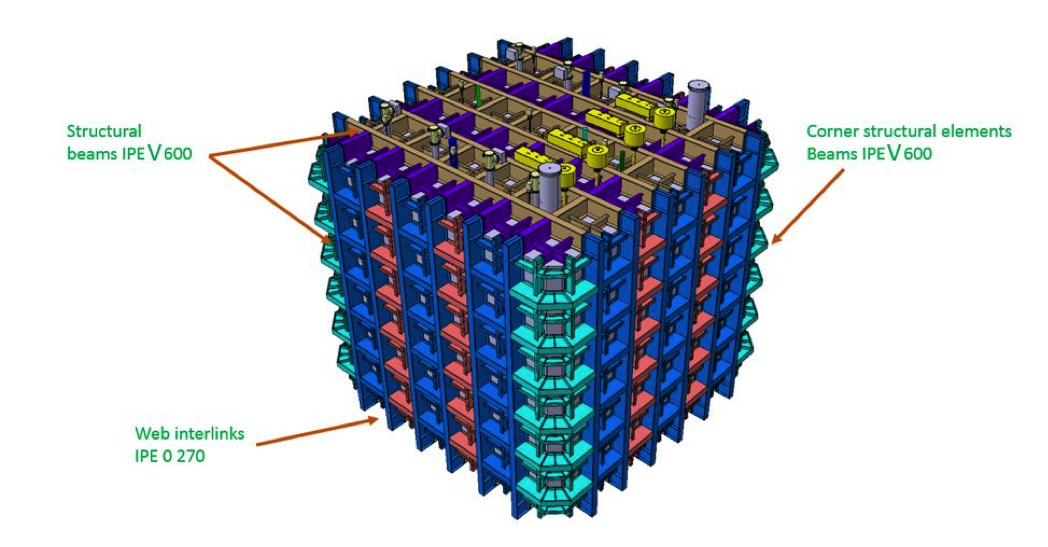
\includegraphics[width=1.\textwidth]{warm-vessel-layout}
\end{cdrfigure}
Inside the steel structure, a 10-mm thick skin of stainless steel plates are welded to provide a gas barrier to the outside.
The top of the cryostat is accessible for installation of the detector elements, the electrical/signal feedthrough, the detector supports and other cryogenics services.  The dimensions %requirements 
are dictated by the required %need to provide a sufficient 
active volume of LAr, constraints on the distances from the active volume to the cryostat inner walls and cryostat material thicknesses.  % to the detector. This means a transversal internal dimension of the liquid volume of 
The inner cryostat dimensions are: width = 8.548~m, length = 8.548~mm and height = 7.900~m. The dimensions 
%\fixme{of the active volume or total volume (which would equal the entire volume inside the membrane)?} %have been adapted in order to 
ensure that all crossing penetrations are arranged as requested and that there is enough space for maintenance. 
%\fixme{Does this mean: the dimensions of the active LAr volume take into account the volume taken up by penetrations in the roof? Are pipes and cables and such allowed to penetrate the active volume? I assume not the fiducial volume...?} 


A secondary membrane is located within the insulation layer. The cold vessel is based on the GTT membrane technology~\cite{gtt}.   Thermal requirements call for 
a thickness of 800\,mm, including the insulation, and the primary and secondary membranes. These two membranes provide a first and second level of containment. There is no requirement at this point for additional containment at the level of the warm steel structure. The SS skin of 10-mm thickness between the warm structure and the insulation provides an effective gas enclosure, which allows control of the argon atmosphere inside the insulation volume.
All necessary information can be found in~\cite{edms1}. 
The 3D detailed CAD model is visible in~\cite{edms2}. 

Prior to installation of the GTT insulation and %cold liquid 
inner membranes, the gas tightness of the SS 10-mm membrane will be measured and verified by CERN using dye penetrant analysis, local vacuum-bag techniques, and He leak %leaks sniffing 
detection at the level of the natural He present in the atmosphere ($\sim2-3 \times 10^{-6} mbar/l/sec$). A report will be presented to GTT.

%%%%%%%%%%%%%%%%%%%%%%%%%
\subsection{Storage characteristics}


The 
cryostat is required to store LAr at a temperature between 86.7\,K and 87.7\,K with a pressure inside the 
tank of 950 < P < 1100\,mbar. %A special emphasis has been made on the thermal fluxes. 
The thermal fluxes must be tightly controlled, i.e., %They must be controlled and 
they will be kept under 5\,W/m2 on %the walls/floor 
the inner membrane that is in contact with liquid, in order to prevent boiling of the LAr.

The storage parameters of the cryostat are as follows:
%\fixme{I changed this from enumerate to itemize; this isn't really an ordered list.}
\begin{itemize} % Need  \usepackage{enumerate} to append this: [(a)]
\item The inner dimensions are 7900\,mm high $\times$ 8548\,mm length $\times$ 8548\,mm wide.  This corresponds to a total volume of $\sim$580 m$^3$. 
\item Tank liquid capacity (assuming a $\sim$4\% ullage): $\sim$ 557 m$^3$
\item Residual Heat Input (RHI): 5-6\,W/m$^2$
\item Insulation weight: 90 kg/m$^3$  
\item Insulation thickness (all included): 0.8\,m 
\item Design pressure: Max \SI{1350} mBar / Min 950 mBar.  The \SI{1350} mBar is for an accident condition during the cryogenics operation.
\item Operating temperature: 86K-89\,K
\end{itemize}

Figure~\ref{fig:cryo-overall-dim} shows a side cross section of the cryostat with the inner dimensions of the cryostat, 
%dimensions of the \SI{10}{mm} SS skin 
the thickness of the insulation 
and the overall outer dimensions of the warm structure.
%\fixme{It only shows in 2D}

\begin{cdrfigure}[Cryostat overall dimensions]{cryo-overall-dim}{Cryostat overall dimensions}
  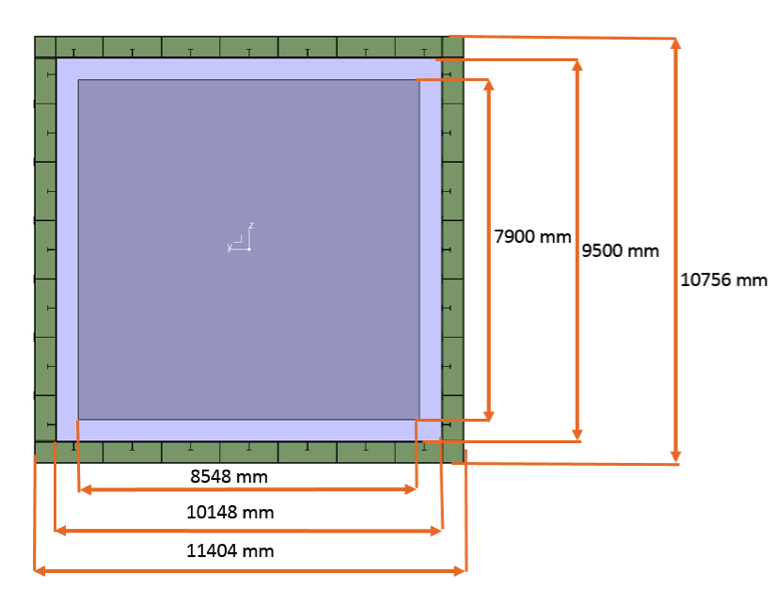
\includegraphics[width=0.8\textwidth]{cryo-overall-dim}
\end{cdrfigure}


%%%%%%%%%%%%%%%%%%%%%%%%%
\subsection{Cold GTT vessel}

The GTT cold vessel is installed inside the warm support structure, which includes the stainless steel gas enclosure membrane. The cold vessel consists of a thermal insulation, a primary corrugated stainless steel membrane, as well as a secondary thin membrane, to provide primary and secondary liquid containment. A cross sectional view of the insulation and membrane layers is shown in Figure~\ref{fig:xsec-insulation-layers}.

\begin{cdrfigure}[Cross section of insulation layers on membranes]{xsec-insulation-layers}{Cross section of insulation layers on membranes}
  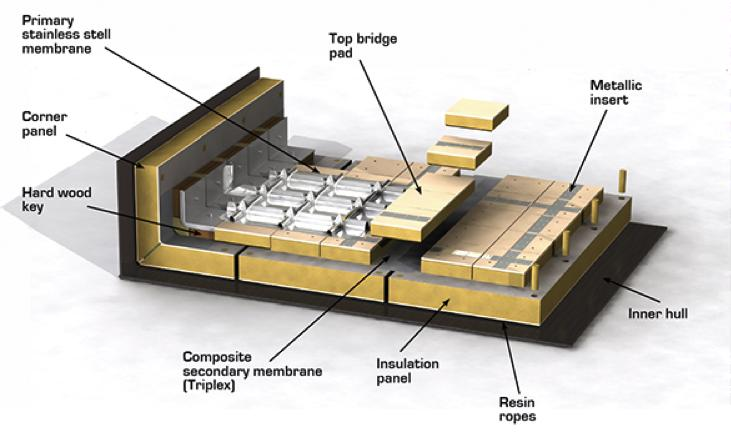
\includegraphics[width=0.8\textwidth]{xsec-insulation-layers}
\end{cdrfigure}


The primary membrane is made of corrugated stainless steel 304 L and is 1.2 mm in thickness.  The standard size of the sheets is 3\,m $\times$ 1\,m.  The secondary membrane is made of Triplex.  This is a composite laminated material of a thin sheet of aluminium between two layers of glass cloth and resin.  It is positioned inside the prefabricated insulation panels between two of the insulation layers.    The insulation is made from reinforced polyurethane foam.  The insulation panels are bonded to the inner 10 mm skin using resin ropes.  The insulation layers are instrumented with gas inlets, outlets, temperature and pressure sensors.


%%%%%%%%%%%%%%%%%%%%%%%%%
\subsection{Temporary Construction Opening (TCO)}

A dedicated access window is necessary to install the ProtoDUNE-SP detector.  This is referred to as the temporary construction opening (TCO) and shown in Figure~\ref{fig:front-tco-np04}.  This means that no insulation of membrane can be installed at the beginning in this location. Once the detector installation has progressed as far as possible and all of the large TPC components are inside the cryostat, the TCO will be closed.  The 10-mm SS skin, insulation and cold membranes are installed and welded in place. 

\begin{cdrfigure}[Front view of the cryostat with the TCO for the NP04 cryostat]{front-tco-np04}{Front view of the cryostat with the TCO for the NP04 cryostat shown in green.}
  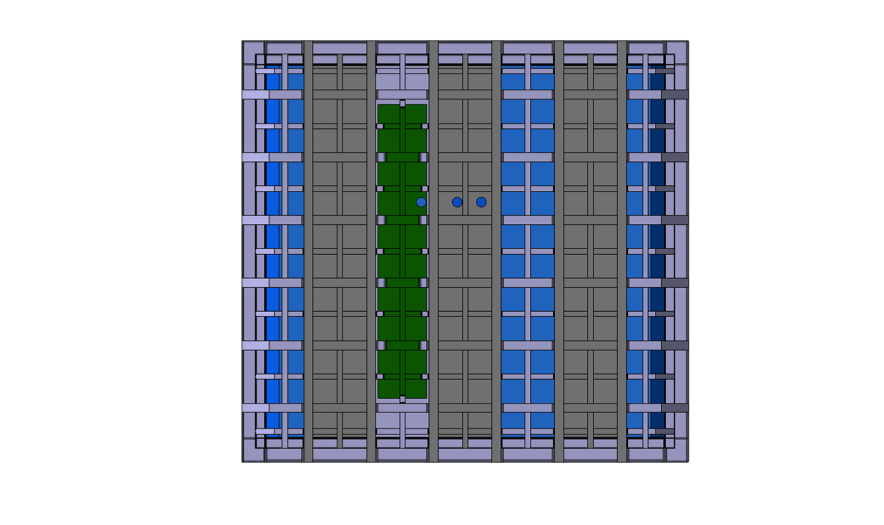
\includegraphics[width=0.8\textwidth]{front-tco-np04}
\end{cdrfigure}


%%%%%%%%%%%%%%%%%%%%%%%%%
\subsection{LAr pump penetration}

To keep the high level of purity required, LAr is extracted from a point as low as possible in the cryostat and pushed by cryo-pumps 
to the external filtering system through the liquid recirculation circuit. A special penetration is thus 
%foreseen 
required on one side wall of the cryostat to connect through a dedicated system of safety valves to the liquid argon pumps.
%On one side wall, as low as possible, a special penetration is foreseen to connect the extraction liquid argon pumps that will allow the liquid recirculation to an external filtering system. To keep the high level of purity required, an external pump is connected on one side to the bottom of the liquid, through a dedicated system of safety valves. 
This penetration requires a local modification of the insulation panels and the SS primary membrane, and consists of a crossing tube with a diameter of 168\,mm for the insulation and the membrane, and a larger-diameter hole at the stainless steel plate.

%%%%%%%%%%%%%%%%%%%%%%%%%
\subsection{Beam window penetration}
\label{subsec:beamwindow}
%%%\fixme{Paola needs to update this section to describe the CERN beam penetration design}
Once constructed, the ProtoDUNE-SP detector will be exposed to the charged
particle beam from the SPS accelerator. To minimize energy loss and
multiple scattering of the beam particles in the dead material of the
cryostat and its insulation, a beam window is inserted at the primary beam position as defined  in Section~\ref{sec:beamrequirements}. 

  The vacuum pipe of the beamline has an external diameter of 219~mm. The beam window is being designed with a dimension of 250~mm in diameter to allow for alignment tolerances.  The direction of the beam window follows the one of the beam.
The outer portion of the
beam window penetration is a vacuum pipe that extends from the H4 beamline (see Section~\ref{sec:h4beamline})  through the outer insulation layer and ends at the secondary
membrane. A safety valve at the cryostat entrance ensures fast segmentation of the vacuum in case of accident.   The
portion of the foam insulation between the secondary and the primary
membrane is replaced with a lower density foam %(9~kg/cm$^3$).
(9~kg/m$^3$).
To maintain structural integrity, the plywood supporting
the primary membrane in the vicinity of the beam window penetration is
replaced with a Nomex honeycomb plate sandwiched between thin G10 or Carbon layers. Nomex is a polymer material with high thermal resistance and Nomex sandwiches are well known for their structural resistance, and have already been used at cryogenic temperatures in the ATLAS detector.
 In this design, both the
primary and secondary stainless steel membranes remain intact. Care has been taken to position the beam window exit on the interior of the cryostat to match a flat section of the corrugated primary SS membrane.
Thermal and stress analyses are being conducted in collaboration with GTT. These will influence the detailed design of the first segment of the beam window. 
The total amount of material in this design, including the primary membrane, and assuming a 0.3~mm G10 thickness on both sides of the Nomex sandwich and a 0.3-mm-thick steel beam window, is equivalent to 10\% of a radiation length. 

%%%%%%%%%%%%%%%%%%%%%%%%%
\subsection{Roof signal, services and supports penetrations}

The penetrations through the cryostat have been arranged by position and diameter. %(see Section 8). 
Most of the penetrations are placed on the ceiling of the cryostat. They have been differentiated into two main groups according to their function and the thermal stresses they will be submitted to. The classification determines whether penetrations can be used to support the weight of the detector or not.
The penetrations on the roof of the NP04 cryostat are detailed in Table~\ref{tab:roofpenetrations}.  
A 3D CAD model to identify all positions can be found at~\cite{edms4} and in an associated drawing~\cite{edms5}.


\begin{cdrtable}[Cryostat penetrations, roof]{llll}{roofpenetrations}{Cryostat penetrations in roof and on side.}
Component &  Quantity & Value \\ \toprowrule
West TPC translation suspension:  & crossing tube diameter & \SI{200}{mm}\\ \colhline
Center TPC translation suspension: & crossing tube diameter & \SI{200}{mm}\\ \colhline
East TPC translation suspension: & crossing tube diameter & \SI{200}{mm}\\ \colhline
Signal cable chimney FTs:& crossing tube diameter & \SI{250}{mm}\\ \colhline
Spare on Signal cable row FTs: & crossing tube diameter & \SI{250}{mm}\\ \colhline
Laser FTs: &  crossing tube diameter & \SI{160}{mm}\\ \colhline
Calibration Fiber CPA FT:&  crossing tube diameter & \SI{250}{mm}\\ \colhline
Spare on CPA line FTs:&  crossing tube diameter & \SI{150}{mm}\\ \colhline
HV FT: &  crossing tube diameter & \SI{250}{mm}\\ \colhline
Manhole:&   crossing tube diameter & \SI{710}{mm}\\ \colhline
Angled beam windows -- west side:&   crossing tube diameter & \SI{250}{mm}\\ \colhline
 &   Vertical: \SI{11.342}{\degree} & \\ \colhline
 &    Horizontal: \SI{11.844}{\degree} & \\ \colhline
TCO - side:&   \num{1200}\si{mm} $\times$ \num{7300}\si{mm} & \\ \colhline
 Cryogenic pipes - roof: &    & \\ \colhline
 &   crossing tube diameter & \SI{250}{mm}\\ \colhline
 &   crossing tube diameter & \SI{304}{mm}\\ \colhline
 &  crossing tube diameter & \SI{152}{mm}\\ \colhline
 &   crossing tube diameter & \SI{125}{mm}\\ \colhline
 &   crossing tube diameter & \SI{250}{mm}\\ \colhline
 Cryogenic pipes -- north side: &  crossing tube diameter & \SI{168}{mm}\\ 
\end{cdrtable}

%%%%%%%%%%%%%%%%%%%%%%%%%
%\subsection{Mechanical mounts and supports}
\subsection{Detector Support Structure (DSS)}


Prior to the installation of the TPC, the detector support structure DSS is installed inside the cryostat.  The DSS is shown in Figure~\ref{fig:dss-install}.  It is positioned near the ceiling and is supported by nine penetrations through the cold side of the membrane extending up to the warm structure of the cryostat.  The warm structure of the cryostat supports all of the loads from the detector.  The DSS consists of two layers of I beams.  The top (yellow) layer is oriented in the y direction and designated as the Y beams and the bottom (purple) layer is oriented in the x direction and designated as the X beams. \\
The Y beams are fixed in the y direction at the center support point, but free to move during the cool down at the two outer points.  The ends of the Y beams are expected to shrink $\sim$10\,mm towards the center during cooldown to LAr temperature.  

The X beams are used for the direct support and positioning of the TPC components.  Only three X beams are shown in Figure~\ref{fig:dss-install}, but there are two additional inbetween the ones shown.  
The full set of beams is shown in Figure~\ref{fig:dss-install2} along with the naming convention for the X beams.
 X beam A supports the row of APAs near the Saleve side of the cryostat.  X beam B is used for the installation and support of the end wall FC in the Saleve drift of the cryostat.  X beam C supports the row of CPAs.  X beam D is used for the installation and support of the end wall FC in the Jura drift.  X beam E supports the row of APAs near the Jura side of the cryostat.  

The X beams have the ability to translate on rolling trolleys in the Y direction in order to move the TPC components from the TCO entrance to their correct position in Y inside the cryostat.  They are fixed in the X direction to the Y beams at the beam side of the cryostat.  The reason 
to fix the X beams on the beam side is to limit the movement of the beam side of the TPC with respect to the membrane wall since
the beam plug is mounted at this side of the TPC.  

\begin{cdrfigure}[Detector support system]{dss-install}{Detector support system}
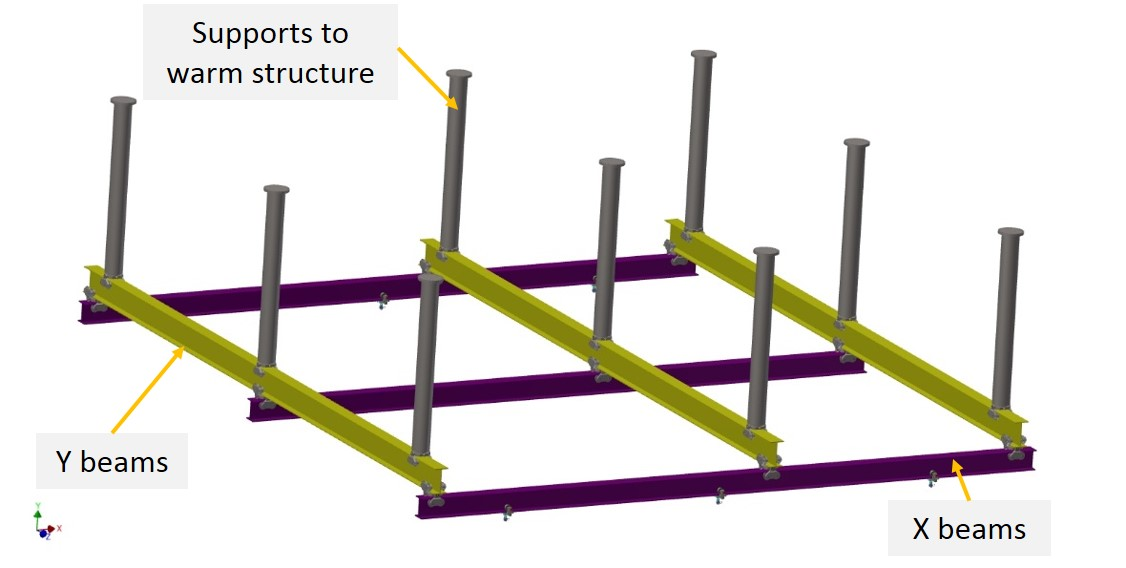
\includegraphics[width=0.8\textwidth]{detector-support-system-xy}
\end{cdrfigure}

\begin{cdrfigure}[DSS showing full set of beams]{dss-install2}{DSS showing full set of beams; the horizontal (X) beams in the figure are called \textit{bridge beams} and the vertical (Y) beams are called \textit{runway} beams. }
 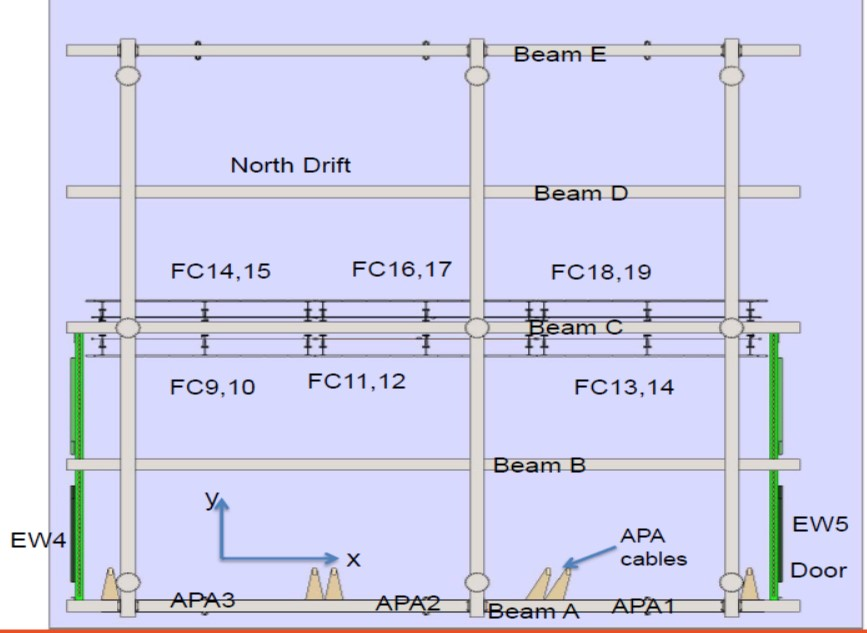
\includegraphics[width=0.6\textwidth]{dss-full-set-of-beams}
\end{cdrfigure}

\fixme{Anne updated the caption for Figure~\ref{fig:dss-install2} per Bill Miller 2/16/17}